\documentclass[dvisvgm]{minimal}
\usepackage{tikz}
\usetikzlibrary{shapes.geometric,arrows.meta,positioning,calc}

\begin{document}
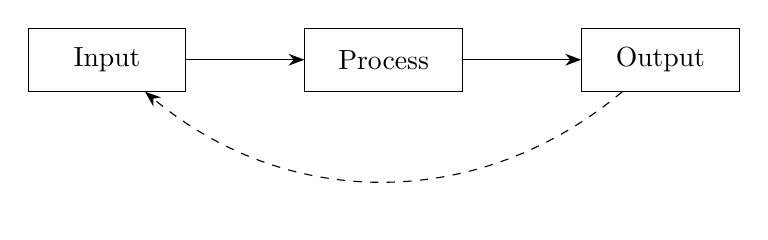
\begin{tikzpicture}[
  box/.style={rectangle, draw, minimum width=2cm, minimum height=0.8cm},
  arrow/.style={-{Stealth[length=2mm]}}
]
  \node[box] (input) {Input};
  \node[box, right=1.5cm of input] (process) {Process};
  \node[box, right=1.5cm of process] (output) {Output};
  \draw[arrow] (input) -- (process);
  \draw[arrow] (process) -- (output);
  \draw[arrow,dashed] (output) to[bend left=40] (input);
\end{tikzpicture}
\end{document}
